

Recently computer vision has made great progress by training deep
feedforward neural networks on large labeled datasets.
However, acquiring labeled training data for all of the problems that
we care about is expensive.
Furthermore, some problems require top-down inference as well as
bottom-up inference in order to handle ambiguity.
For example, consider the problem of object detection
and instance segmentation (cf. \cite{Hariharan2014})  in the
presence of clutter/occlusion. 

\begin{wrapfigure}[11]{r}[12pt]{6cm}
\vspace{-4mm}
\begin{center}
    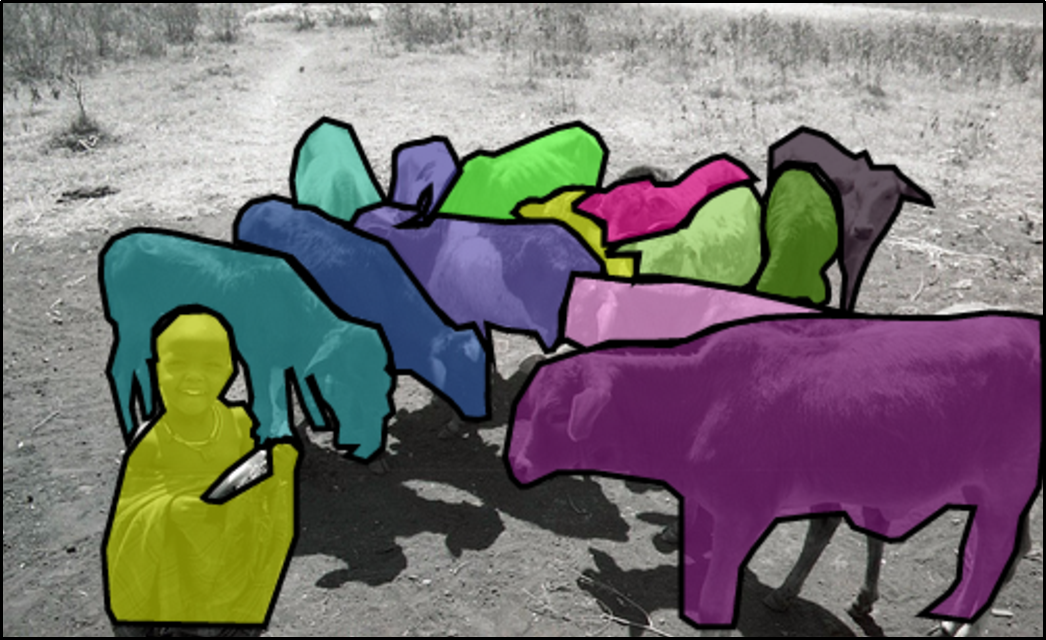
\includegraphics[width=0.375\textwidth]{figs/cows.pdf} \vspace{-2mm}
    \caption{\footnotesize Some cows}
    \label{fig:cows}
  \end{center}
  \vspace{-2mm}
\end{wrapfigure}
In this case, the foreground object may
obscure almost all of the background object, yet people are still able
to detect that there are two objects present, to correctly segment
out both of them, and even to amodally complete the hidden parts of
the occluded object (cf., \cite{Kar2015}).
\Kevin{Jon, can you add your image of occluded cows to illustrate this?}


One way to tackle this problem is to use generative models.
In particular, we can imagine the following generative process for an image:
(1) Choose an object (or texture) of interest, by sampling a ``content vector''
representing its class label, style, etc;
(2) Choose where to
place the object in the 2d image plane, by sampling a ``pose vector'',
representing location, scale, etc. 
(3) Render an image of the object onto a hidden canvas or layer;
\Kevin{The term layer could refer to a hidden image or a hidden layer
  in the neural network...}
(4) Repeat this process for $N$
objects (we assume in this work that $N$ is fixed);
(5) Finally, generate
the observed image by compositing the layers in order.\footnote{
%
There are many  ways to composite multiple layers in computer
graphics~\citep{porter1984compositing}. 
In our experiments, we use  the classic \emph{over operator}, which
reduces to a simple $\alpha$-weighted 
convex combination of foreground and background pixels,
in the two-layer setting.
 See Section~\ref{sec:models} for more details.
}

There have been several previous attempts to use layered generative
models to perform scene parsing and object detection in clutter (see
Section~\ref{sec:related} for a review of related work). However, such
methods usually run into computational bottlenecks, since inverting
such generative models is intractable.
In this paper, we build on recent work (primarily \cite{Kingma2014,gregor2015draw})
that shows how to jointly train a generative model and an inference
network in a way that optimizes a variational lower bound on the log
likelihood of the data;
this has been called a ``variational auto-encoder'' or VAE.
In particular, we extend this prior work in
two ways. First, we extend it to the sequential setting, where we
generate the observed image in stages by compositing hidden layers
from back to front. \Jon{we have to be a bit careful about claiming this}
Second, we combine the VAE with the spatial transformer network of
\citep{jaderberg2015spatial}, which allows us to factor out variations
in pose (e.g., location) from variations in content (e.g., identity).
We call our model the ``composited spatially transformed VAE'', or CST-VAE
for short.

Our resulting inference algorithm combines top-down (generative)
and bottom-up (discriminative) components in an interleaved fashion as follows:
(1)  First we recognize (bottom-up) the foreground object, factoring apart pose and content;
(2) Having recognized it, we generate (top-down) what hidden image 1 should look
like;
(3) Finally, we virtually remove this generated hidden image from the observed
image to get the residual image, and we repeat the process.
(This is somewhat reminiscent of approaches that the brain is believed
to use, \cite{Hochstein2002}.)

The end result is a way to factor an observed image of
overlapping objects into $N$
hidden layers, where each layer contains a single object
with its pose parameters.
Remarkably, this whole process can be trained in a fully unsupervised
way using standard gradient-based optimization methods
(see Section~\ref{sec:models} for details).
In Section~\ref{sec:eval}, we show that our method is able to reliably
interpret cluttered images, and that the inferred latent
representation is a much better  feature vector for a discriminative
classification task than working with the original cluttered images.




\eat{
Large strides have been made in computer vision in recent years 
due to scalable deep learning and massive labeled datasets such as Imagenet~\cite{krizhevsky2012imagenet,deng2009imagenet}.
But as we move beyond simple image classification problems to more complication output spaces, the limitations
to our current approaches are becoming more transparent.
Dense labeling problems such as semantic segmentation, instance segmentation, for example,
require much more human effort per image to label and more images in general.




We've seen less progress on unsupervised models  ---  using MCMC

traditional graphical models from yesteryear (citations?) 	- methods tend to be less scalable often requiring intractable normalization constants to be computed
  --- recent work has bypassed this (citations) allowing models to be trained via gradient methods


Things don't just have one label

We also are starting to get interested in dense labels of images and video: think semantic segmentations, instance level segmentations, depth, etc.
	It's getting more and more expensive to collect this data.

	
Unsupervised and weakly supervised models are the next frontier.  

The goal is to model the variation in real images.  
Disentangling the factors of variation is critical to confronting the curse of dimensionality.

conv nets for example learn higher levels of abstraction, disentangling variation in appearance

there has been some work in the deep learning community factoring pose from appearance.

No work on factoring out the variability stemming from Multiple objects.

We propose a layered model of image generation.  And it has these benefits.


\Jon{play up interpretability of the model}


A critical issue in counting and instance level segmentation is dealing with things that can overlap and partially occlude each other, and current detection methods that use non-max suppression, for example, are not smart at reasoning about overlap/occlusion.  

In the instance segmentation problem, for example, we might need to analyze a local patch and decide whether it belongs to instance A, or instance B, or whether there were even two instances that were overlapping to begin with.  In some of these settings, the decision cannot be made at the local level and requires a global understanding of the semantics of the scene.


Motivations:
	The idea that we explore here is: if we only knew what the instances A and B were supposed to look like (i.e., had pixel-level generative models of A and B), we would be better positioned to make this decision.

	Being able to do this can help in a ton of applications: counting, instance segmentation
		even training for object recognition ? a lot of examples are occluded and if knew how
			how to factor out this variation, it could help
			
	But we can go further: we can imagine what?s behind (amodal completion)

	A step toward integrating top-down and bottom-up
	
	part of the story is that we're able to use VAEs to now combine some of the prior structure that we know about 
		with the rich expressiveness of deep models and train them all together with backprop

We propose a generative model that separately generates a ?layer? for each object in the image
in which each layer itself we?ve separated pose from style.
\begin{itemize}
\item fully unsupervised training (?) using ordinary sgd based methods that use backprop
\item st-aevb model
\item new ?alpha compositing? layer which is kind of like a pixelwise attention mechanism
\item masked inference mechanism allowing for training from partially observed images
\item usage of conv and deconv layers in a fully probabilistic generative model
\item show how to reason with occlusions and do amodal completion of objects based on a generative model
can handle multiple and unknown number of objects?
\end{itemize}
}